
\documentclass[usenames,dvipsnames,svgnames]{beamer}

\usepackage[utf8]{inputenc}
\usepackage{lmodern}
\usepackage{array} % needed for \arraybackslash
\usepackage{graphicx}
\usepackage{adjustbox} % for \adjincludegraphics
\usepackage{amsmath}
\usepackage{tikz}
\usepackage{tkz-euclide}
\usepackage[portuguese]{babel}

%Information to be included in the title page:
\title{Conjuntos Numéricos: $\mathbb{N}, \mathbb{Z}, \mathbb{Q}, \mathbb{R}, \mathbb{C}$}
\author{Matemática}
\institute{ONGEP}
\date{2018}

\begin{document}

\frame{\titlepage}

\begin{frame}	
	\frametitle{Notas Históricas}
	\framesubtitle{Números Naturais: $\mathbb{N}$}

	\begin{columns}[t]
	\begin{column}{.25\textwidth}
		\begin{figure}
			\adjincludegraphics[width=.9\linewidth,valign=t]{pictures/Ishango}
			\caption{\small Osso de Ishango (18.000~AC -- 20.000~AC)}
		\end{figure}
	\end{column}
	\begin{column}{.75\textwidth}
		\begin{itemize}
		\item Com o advento da linguagem, surgiu a necessidade de comunicar quantidades numéricas a um interlocutor
		\item A maneira mais primitiva de representação de um número natural consiste em denotá-lo por um conjunto de marcações (p.ex. $5 = \circ \circ \circ \circ \circ$)
		\item Ainda que limitada, a representação por marcações permite testar relações de equalidade, excesso (``maior que'', $>$) e deficiência (``menor que'', $<$) entre dois números
		\item Exemplo: $\circ \circ \bullet \bullet \bullet | \bullet \bullet \bullet$, logo $5 > 3$
		\end{itemize}
	\end{column}
	\end{columns}
\end{frame}

\begin{frame}	
	\frametitle{Notas Históricas}
	\framesubtitle{Números Naturais: $\mathbb{N}$}

	\begin{columns}[t]
	\begin{column}{.3\textwidth}
		\begin{figure}
			\adjincludegraphics[width=1\linewidth,valign=t]{pictures/numeral_systems}
			\caption{\small Sistemas de numerais arábicos ocidentais, arábicos orientais, Romanos, Benengaleses, Tamil, Khmer e Chineses, em ordem}
		\end{figure}
	\end{column}
	\begin{column}{.7\textwidth}
		\begin{itemize}
		\item O primeiro avanço em termos de {\color{red}abstração} foi a representação numérica usando \emph{numerais} (Figura ao lado)
		\item A representação compacta ($60$ vs \tiny$\circ \circ \circ \circ \circ \circ \circ \circ \circ \circ \circ \circ \circ \circ \circ \circ \circ \circ \circ \circ \circ \circ \circ \circ \circ \circ \circ \circ \circ \circ \circ \circ \circ \circ \circ \circ \circ \circ \circ \circ \circ \circ$\normalsize) nos convida a desenvolver {\color{red}notações} para denotar operações aritiméticas importantes ($+, -, \times, \div$)
		\item Desse modo, a abstração nos convida a fazer perguntas inicialmente proibidas: $5 - 8 = ?$
		\item A tentativa de responder essas perguntas promove a {\color{red}generalização} dos conceitos. Esse é o motor do desenvolvimento da matemática.
		\end{itemize}
	\end{column}
	\end{columns}	
\end{frame}

\begin{frame}	
	\frametitle{Números Naturais: $\mathbb{N}$}

	\begin{itemize}
		\item A expressão $5 - 8$ é \emph{proibida} nos números naturais, ou, no linguajar matemático: \\ ``\emph{A expressão não admite soluções em $\mathbb{N}$}''
		\item Na notação de teoria dos conjuntos: ${\color{red}5-8}~{\color{ForestGreen}\not\in}~{\color{blue}\mathbb{N}}$
		\item O símbolo $\in$ denota {\color{ForestGreen}pertinência} a um conjunto. ${\color{red}x}~{\color{ForestGreen}\in}~{\color{blue}\mathbf{A}}$ se lê, em português: \\ ``{\color{red}o elemento x} {\color{ForestGreen}faz parte do}  {\color{blue} conjunto A}''
		\item A versão ``riscada'' de $\in$, $\not\in$, denota o oposto: ``não pertence''.
	\end{itemize}
\end{frame}

\begin{frame}	
	\frametitle{Números Naturais: $\mathbb{N}$}

	\begin{itemize}
		\item Quais elementos fazem parte de $\mathbb{N}$? \\ R: $0, 1, 2, 3, \dots$
		\item OK, mas \emph{concretamente}, o que tá escondido em $\dots$? Como a gente sabe o que vem depois do $3$? Podíamos ter parado no $2$? No $1$? Quantas enumerações são suficientes?
		\item Em resumo, como {\color{red}definir} o conjunto $\mathbb{N}$?
		\item Bom, $0 \in \mathbb{N}$.
		\item O que mais? Nós queremos expressar a ideia de que $\mathbb{N}$ é {\color{red}infinito}.
		\item Como, intuitivamente, nós sabemos que $\mathbb{N}$ é infinito?
 	\end{itemize}
\end{frame}

\begin{frame}	
	\frametitle{Números Naturais: $\mathbb{N}$}

	\begin{itemize}
		\item $\mathbb{N}$ é inifnito porque não existe o ``maior número'' de $\mathbb{N}$
		\item Por quê?
		\item Me dá um candidato $n$ a maior número que eu te dou um número maior
		\item Qual?
 	\end{itemize}
\end{frame}

\begin{frame}	
	\frametitle{Números Naturais: $\mathbb{N}$}

	\begin{itemize}
		\item $\mathbb{N}$ é inifnito porque não existe o ``maior número'' de $\mathbb{N}$
		\item Por quê?
		\item Me dá um candidato $n$ a maior número que eu te dou um número maior
		\item Qual?
		\item O ``sucessor'' de $n$: $n+1$
 	\end{itemize}
\end{frame}

\begin{frame}	
	\frametitle{Números Naturais: $\mathbb{N}$}

	\begin{itemize}
		\item OK, isso é suficiente para definir $\mathbb{N}$? Sim!
		\item Definição:
		\item
			\begin{equation}
			\begin{aligned}
				0 \in \mathbb{N} \\
				\textrm{Para todo $n \in \mathbb{N}$:} ~~ n+1 \in \mathbb{N}
			\end{aligned}
			\end{equation}
		\item
			\begin{equation}
			\begin{aligned}
				0 \in \mathbb{N} \\
				\forall n \in \mathbb{N}: ~~ n+1 \in \mathbb{N}
			\end{aligned}
			\end{equation}
		\item O símbolo $\forall$ denota ``para todo''. A expressão ${\color{RoyalPurple}\forall}{\color{red}x}~{\color{ForestGreen}\in}~{\color{blue}\mathbf{A}}$ se lê, em português: \\
		``{\color{RoyalPurple} para todo} {\color{red}elemento $x$} {\color{ForestGreen} que pertence ao} {\color{blue}conjunto $\mathbf{A}$}''
 	\end{itemize}
\end{frame}

\begin{frame}	
	\frametitle{Números Inteiros: $\mathbb{Z}$}

	\begin{itemize}
		\item Voltando à pergunta: $5 - 8 = ?$
		\item Se $5 - 8 \not\in \mathbb{N}$, a que conjunto $5 - 8$ pertence? Qual o conjunto $\mathbf{A}$ pro qual podemos escrever $5 - 8 \in \mathbf{A}$?
		\item Recorremos à {\color{red}generalização}: vamos generalizar a subtração para que $5 - 8$ seja uma expressão bem definida!
		\item OK, como?
 	\end{itemize}
\end{frame}

\begin{frame}	
	\frametitle{Números Inteiros: $\mathbb{Z}$}

	\begin{itemize}
		\item A justificativa histórica para os números negativos é o conceito de {\color{red}débito}. Um comprador que deve 8 reais a um comerciante, mas só tem 5 no bolso, fica \emph{devendo} $8 - 5 = 3$ reais.
		\item Esse ponto é chave: o débito é calculado trocando os números de lugar! A transação $5 - 8$ produz $3$ de débito.
		\item A notação que usamos pra débito na matemática é o conceito de \emph{negativo}: $5 - 8 = -3$, ou, em português: ``cinco menos oito é igual a três negativo''
		\item Eis o conceito de {\color{red}simetria}: a subtração não é comutativa ($5-8 \neq 8-5$), mas é {\color{red}quase}: só muda o sinal!
		\item Exemplo: $5-8=-3$ e $8-5=3$ 
 	\end{itemize}
\end{frame}

\begin{frame}	
	\frametitle{Números Inteiros: $\mathbb{Z}$}

	\begin{columns}[t]
	\begin{column}{.3\textwidth}
		\begin{figure}
			\adjincludegraphics[width=1\linewidth,valign=t]{pictures/Cicada}
			\caption{\small Anatomia de uma Cigarra, um animal com simetria bilateral (clado \emph{bilateria} na biologia)}
		\end{figure}
		\begin{figure}
			\small $-3, -2, -1, ~0, ~1, ~2, ~3$
			\caption{\small Linha numérica de $\mathbb{Z}$}
		\end{figure}
	\end{column}
	\begin{column}{.7\textwidth}
		\begin{itemize}
		\item Uma maneira de definir o sinal ``$-$'' que colocamos na frente dos números negativos é a seguinte: $\forall n: (-n) + n = 0$
		\item Em resumo: $-n$ denota $n$ passos à esquerda e $n$ denota $n$ passos à direita na linha numérica
		\item A esquerda e à direita da onde?
		\end{itemize}
	\end{column}
	\end{columns}
\end{frame}

\begin{frame}	
	\frametitle{Números Inteiros: $\mathbb{Z}$}

	\begin{columns}[t]
	\begin{column}{.3\textwidth}
		\begin{figure}
			\adjincludegraphics[width=1\linewidth,valign=t]{pictures/Cicada-axis}
			\caption{\small Anatomia de uma Cigarra, um animal com simetria bilateral (clado \emph{bilateria} na biologia)}
		\end{figure}
		\begin{figure}
			\small $-3, -2, -1, ~{\color{red}0}, ~1, ~2, ~3$
			\caption{\small Linha numérica de $\mathbb{Z}$}
		\end{figure}
	\end{column}
	\begin{column}{.7\textwidth}
		\begin{itemize}
		\item Uma maneira de definir o sinal ``$-$'' que colocamos na frente dos números negativos é a seguinte: $\forall n: (-n) + n = 0$
		\item Em resumo: $-n$ denota $n$ passos à esquerda e $n$ denota $n$ passos à direita na linha numérica
		\item A esquerda e à direita da onde?
		\item {\color{red}De $0$!}
		\item $0$ é o {\color{blue}eixo de simetria} da relação de negação, assim como o ponto médio (horizontal) da Figura ao lado é o eixo de simetria (bilateral) da cigarra
		\end{itemize}
	\end{column}
	\end{columns}
\end{frame}

\begin{frame}	
	\frametitle{Números Inteiros: $\mathbb{Z}$}

	\begin{columns}[t]
	\begin{column}{.3\textwidth}
		\begin{figure}
			\adjincludegraphics[width=1\linewidth,valign=t]{pictures/Cicada}
			\caption{\small Anatomia de uma Cigarra, um animal com simetria bilateral (clado \emph{bilateria} na biologia)}
		\end{figure}
		\begin{figure}
			\small $-3, -2, -1, ~0, ~1, ~2, ~3$
			\caption{\small Linha numérica de $\mathbb{Z}$}
		\end{figure}
	\end{column}
	\begin{column}{.7\textwidth}
		\begin{itemize}
		\item Poderíamos definir outro eixo de simetria? Sim, múltiplos: \\ $\forall n: (-n) + n = 1$ \\ $\forall n: (-n) + n = -387$ \\ $\forall n: (-n) + n = 42$ \\ $\dots$
		\item Quantos? Um para cada número $\in \mathbb{Z}$
		\end{itemize}
	\end{column}
	\end{columns}
\end{frame}

\begin{frame}	
	\frametitle{Números Inteiros: $\mathbb{Z}$}

	\begin{itemize}
		\item Nós definimos o conjunto dos números naturais, $\mathbb{N}$, usando a operação de soma
		\item Qual operação precisamos adicionar ao nosso repertório para definir o conjunto dos números inteiros, $\mathbb{Z}$?
 	\end{itemize}
\end{frame}

\begin{frame}	
	\frametitle{Números Inteiros: $\mathbb{Z}$}

	\begin{itemize}
		\item Nós definimos o conjunto dos números naturais, $\mathbb{N}$, usando a operação de soma
		\item Qual operação precisamos adicionar ao nosso repertório para definir o conjunto dos números inteiros, $\mathbb{Z}$?
		\item Subtração!
		\item
			\begin{equation}
			\begin{aligned}
				0 \in \mathbb{Z} \\
				\forall n \in \mathbb{Z}: ~~ n+1 \in \mathbb{Z} \\
				\forall n \in \mathbb{Z}: ~~ n-1 \in \mathbb{Z}
			\end{aligned}
			\end{equation}
 	\end{itemize}
\end{frame}

\begin{frame}	
	\frametitle{O que temos até agora: $\mathbb{N}, \mathbb{Z}$}

	\begin{columns}[t]
	\begin{column}{.4\textwidth}
		\begin{figure}
			\def\Zcircle{		(0,0) 			circle (2.5cm)}
			\def\Ncircle{		(1.25cm:-1.25cm) circle (1.1cm)}
			\def\Zminuscircle{	(1.25cm:1.25cm) circle (1.1cm)}
			\def\Zpluscircle{	(1cm:-1.75cm) circle (0.5cm)}
			\def\zerocircle{	(1.5cm:-0.75cm) circle (0.5cm)}

			% Now we can draw the sets:
			\begin{tikzpicture}
				\draw \Zpluscircle node		[shift={(0,0)}] 	{$\mathbb{Z}^{+}$};
				\draw \zerocircle node		[shift={(0,0)}] 	{$\{0\}$};
				\draw \Ncircle node			[shift={(-0.25cm,0.75cm)}] 	{$\mathbb{N}$};
				\draw \Zminuscircle node	[shift={(0,0)}] 	{$\mathbb{Z}^{-}$};
				\draw \Zcircle node			[shift={(-1.25cm,1.25cm)}] 	{$\mathbb{Z}$};
			\end{tikzpicture}
			\caption{Diagrama de Venn dos conjuntos $\{0\}, \mathbb{Z}^{+}, \mathbb{Z}^{-}, \mathbb{N}, \mathbb{Z}$}
		\end{figure}
	\end{column}
	\begin{column}{.6\textwidth}
		\begin{itemize}
		\item O \emph{Diagrama de Venn} (exemplo à esquerda) é uma maneira de visualizar quais conjuntos {\color{red} estão condidos em} quais outros conjuntos
		\item OBS 1. O tamanho dos círculos não significa nada; $\mathbb{Z}^{+}$ não é ``menor'' que $\mathbb{Z}^{-}$
		\item OBS 2. Num certo sentido, nenhum desses conjuntos (à exceção do $\{0\}$, que é finito) é realmente ``maior'' ou ``menor'' que o outro: todos têm a mesma \emph{cardinalidade} (mais sobre isso mais adiante)
		\end{itemize}
	\end{column}
	\end{columns}
\end{frame}

\begin{frame}	
	\frametitle{O que temos até agora: $\mathbb{N}, \mathbb{Z}$}

	\begin{columns}[t]
	\begin{column}{.4\textwidth}
		\begin{figure}
			\def\Zcircle{		(0,0) 			circle (2.5cm)}
			\def\Ncircle{		(1.25cm:-1.25cm) circle (1.1cm)}
			\def\Zminuscircle{	(1.25cm:1.25cm) circle (1.1cm)}
			\def\Zpluscircle{	(1cm:-1.75cm) circle (0.5cm)}
			\def\zerocircle{	(1.5cm:-0.75cm) circle (0.5cm)}

			% Now we can draw the sets:
			\begin{tikzpicture}
				\draw \Zpluscircle node		[shift={(0,0)}] 	{$\mathbb{Z}^{+}$};
				\draw \zerocircle node		[shift={(0,0)}] 	{$\{0\}$};
				\draw \Ncircle node			[shift={(-0.25cm,0.75cm)}] 	{$\mathbb{N}$};
				\draw \Zminuscircle node	[shift={(0,0)}] 	{$\mathbb{Z}^{-}$};
				\draw \Zcircle node			[shift={(-1.25cm,1.25cm)}] 	{$\mathbb{Z}$};
			\end{tikzpicture}
			\caption{Diagrama de Venn dos conjuntos $\{0\}, \mathbb{Z}^{+}, \mathbb{Z}^{-}, \mathbb{N}, \mathbb{Z}$}
		\end{figure}
	\end{column}
	\begin{column}{.6\textwidth}
		\begin{itemize}
		\item O símbolo $\subset$ denota a relação de ``está contido em''
		\item Por exemplo, $\color{red}\mathbf{A} \color{ForestGreen}\subset \color{blue}\mathbf{B}$ pode ser lido em português como \\ ``{\color{red}O conjunto A} {\color{ForestGreen}está contido no} {\color{blue}conjunto B}''
		\item O símbolo $\supset$ denota a relação inversa: ``contém''
		\item O que podemos dizer sobre $\mathbb{N}, \mathbb{Z}^{+}, \mathbb{Z}^{-}, \mathbb{Z}, \{0\}$, baseado nas suas definições (ou no diagrama ao lado)?
		\end{itemize}
	\end{column}
	\end{columns}
\end{frame}

\begin{frame}	
	\frametitle{O que temos até agora: $\mathbb{N}, \mathbb{Z}$}

	\begin{columns}[t]
	\begin{column}{.4\textwidth}
		\begin{figure}
			\def\Zcircle{		(0,0) 			circle (2.5cm)}
			\def\Ncircle{		(1.25cm:-1.25cm) circle (1.1cm)}
			\def\Zminuscircle{	(1.25cm:1.25cm) circle (1.1cm)}
			\def\Zpluscircle{	(1cm:-1.75cm) circle (0.5cm)}
			\def\zerocircle{	(1.5cm:-0.75cm) circle (0.5cm)}

			% Now we can draw the sets:
			\begin{tikzpicture}
				\draw \Zpluscircle node		[shift={(0,0)}] 	{$\mathbb{Z}^{+}$};
				\draw \zerocircle node		[shift={(0,0)}] 	{$\{0\}$};
				\draw \Ncircle node			[shift={(-0.25cm,0.75cm)}] 	{$\mathbb{N}$};
				\draw \Zminuscircle node	[shift={(0,0)}] 	{$\mathbb{Z}^{-}$};
				\draw \Zcircle node			[shift={(-1.25cm,1.25cm)}] 	{$\mathbb{Z}$};
			\end{tikzpicture}
			\caption{Diagrama de Venn dos conjuntos $\{0\}, \mathbb{Z}^{+}, \mathbb{Z}^{-}, \mathbb{N}, \mathbb{Z}$}
		\end{figure}
	\end{column}
	\begin{column}{.6\textwidth}
		\begin{itemize}
			\item $\{0\} \subset \mathbb{N}$
			\item $\{0\} \not\subset \mathbb{Z}^{+}$
			\item $\mathbb{Z}^{+} \subset \mathbb{N}$
			\item $\mathbb{Z}^{-} \not\subset \mathbb{N}$
			\item $\mathbb{N} \subset \mathbb{Z}$
			\item $\mathbb{Z}^{-} \subset \mathbb{Z}$
		\end{itemize}
	\end{column}
	\end{columns}
\end{frame}

\begin{frame}	
	\frametitle{No caminho da generalização:}
	\framesubtitle{Quais as perguntas proibidas em $\mathbb{Z}$?}

	\begin{itemize}
		\item Escolhe uma operação $(+ / - / \times / \div)$
		\item Escolhe dois números $a \in \mathbb{Z}, b \in \mathbb{Z}$
		\item Consegue criar um número $c \not \in \mathbb{Z}$?
	\end{itemize}

	\begin{equation}
	\begin{aligned}
		c = a ~ (+ / - / \times / \div) ~ b \\
		a \in \mathbb{Z} \\
		b \in \mathbb{Z}
	\end{aligned}
	\end{equation}
\end{frame}

\begin{frame}	
	\frametitle{No caminho da generalização:}
	\framesubtitle{Quais as perguntas proibidas em $\mathbb{Z}$?}

	\begin{itemize}
		\item Escolhe uma operação $(+ / - / \times / {\color{red}\div})$
		\item Escolhe dois números $a \in \mathbb{Z}, b \in \mathbb{Z}$
		\item Consegue criar um número $c \not \in \mathbb{Z}$?
		\item $c = 1 {\color{red}\div} 2$
	\end{itemize}

	\begin{equation}
	\begin{aligned}
		c = a ~ (+ / - / \times / {\color{red}\div}) ~ b \\
		a \in \mathbb{Z} \\
		b \in \mathbb{Z}
	\end{aligned}
	\end{equation}
\end{frame}

\begin{frame}	
	\frametitle{Números Racionais: $\mathbb{Q}$}

	\begin{itemize}
		\item Antes de qualquer coisa: agora que já descobrimos que a operação de interesse é a divisão ($\div$), será que conseguimos definir $\mathbb{Q}$ assim como fizemos com $\mathbb{N}$ e $\mathbb{Z}$?
	\end{itemize}
\end{frame}

\begin{frame}	
	\frametitle{Números Racionais: $\mathbb{Q}$}

	\begin{itemize}
		\item Antes de qualquer coisa: agora que já descobrimos que a operação de interesse é a divisão ($\div$), será que conseguimos definir $\mathbb{Q}$ assim como fizemos com $\mathbb{N}$ e $\mathbb{Z}$?
		\item
		\begin{equation}
		\begin{aligned}
			\substack{\forall n ~\in~ \mathbb{Z} \\ \forall m ~\in~ \mathbb{Z}}: n \div m \in \mathbb{Q}
		\end{aligned}
		\end{equation}
	\end{itemize}
\end{frame}

\begin{frame}	
	\frametitle{Números Racionais: $\mathbb{Q}$}

	\begin{itemize}
		\item Antes de qualquer coisa: agora que já descobrimos que a operação de interesse é a divisão ($\div$), será que conseguimos definir $\mathbb{Q}$ assim como fizemos com $\mathbb{N}$ e $\mathbb{Z}$?
		\item
		\begin{equation}
		\begin{aligned}
			\substack{\forall n ~\in~ \mathbb{Z} \\ \forall m ~\in~ \mathbb{Z}}: n \div m \in \mathbb{Q}
		\end{aligned}
		\end{equation}
		\item Algum problema com essa definição?
	\end{itemize}
\end{frame}

\begin{frame}	
	\frametitle{Números Racionais: $\mathbb{Q}$}

	\begin{itemize}
		\item Antes de qualquer coisa: agora que já descobrimos que a operação de interesse é a divisão ($\div$), será que conseguimos definir $\mathbb{Q}$ assim como fizemos com $\mathbb{N}$ e $\mathbb{Z}$?
		\item
		\begin{equation}
		\begin{aligned}
			\substack{\forall n ~\in~ \mathbb{Z} \\ \forall m ~\in~ \mathbb{Z}}: n \div m \in \mathbb{Q}
		\end{aligned}
		\end{equation}
		\item Algum problema com essa definição?
		\item {\color{red} E se $m = 0$?}
	\end{itemize}
\end{frame}

\begin{frame}	
	\frametitle{Números Racionais: $\mathbb{Q}$}

	\begin{itemize}
		\item Definição corrigida:
		\item
		\begin{equation}
		\begin{aligned}
			\substack{\forall n ~\in~ \mathbb{Z} \\ \forall m ~\in~ \mathbb{Z} \\ {\color{red}m ~\neq~ 0}}: n \div m \in \mathbb{Q}
		\end{aligned}
		\end{equation}
	\end{itemize}
\end{frame}

\begin{frame}	
	\frametitle{Números Racionais: $\mathbb{Q}$}

	\begin{columns}[t]
	\begin{column}{.4\textwidth}
		\begin{figure}
			\def\Ncircle{		(0,0) circle (0.5cm)}
			\def\Zcircle{		(0,0) circle (1.5cm)}
			\def\Qcircle{		(0,0) circle (2.5cm)}

			% Now we can draw the sets:
			\begin{tikzpicture}
				\draw \Ncircle node			[shift={(0,0)}] 		{$\mathbb{N}$};
				\draw \Zcircle node			[shift={(0.7cm,0.7cm)}] {$\mathbb{Z}$};
				\draw \Qcircle node			[shift={(1.4cm,1.4cm)}] 	{$\mathbb{Q}$};
			\end{tikzpicture}
			\caption{Diagrama de Venn dos conjuntos $\mathbb{N}, \mathbb{Z}, \mathbb{Q}$}
		\end{figure}
	\end{column}
	\begin{column}{.6\textwidth}
		\begin{itemize}
			\item $\mathbb{N} \subset \mathbb{Z}$
			\item $\mathbb{Z} \subset \mathbb{Q}$
			\item $\mathbb{N} \subset \mathbb{Z} \subset \mathbb{Q}$
		\end{itemize}
	\end{column}
	\end{columns}
\end{frame}

\begin{frame}	
	\frametitle{No caminho da generalização:}
	\framesubtitle{De novo: Quais as perguntas proibidas em $\mathbb{Q}$?}

	\begin{itemize}
		\item Escolhe uma operação $(+ / - / \times / \div / ~^x, \sqrt[x]{~})$
		\item Escolhe dois números $a \in \mathbb{Q}, b \in \mathbb{Q}$
		\item Consegue criar um número $c \not \in \mathbb{Q}$?
		\item OBS 1. $a ~(~^x)~ b = a^b$
		\item OBS 2. $a ~(\sqrt[x]{~})~ b = \sqrt[a]{b}$
	\end{itemize}

	\begin{equation}
	\begin{aligned}
		c = a ~ (+ / - / \times / \div / ~^x, \sqrt[x]{~}) ~ b \\
		a \in \mathbb{Q} \\
		b \in \mathbb{Q}
	\end{aligned}
	\end{equation}
\end{frame}

\begin{frame}	
	\frametitle{No caminho da generalização:}
	\framesubtitle{De novo: Quais as perguntas proibidas em $\mathbb{Q}$?}

	\begin{itemize}
		\item Escolhe uma operação $(+ / - / \times / \div / ~^x, {\color{red}\sqrt[x]{~}})$
		\item Escolhe dois números $a \in \mathbb{Q}, b \in \mathbb{Q}$
		\item Consegue criar um número $c \not \in \mathbb{Q}$?
		\item OBS 1. $a ~(~^x)~ b = a^b$
		\item OBS 2. $a ~(\sqrt[x]{~})~ b = \sqrt[a]{b}$
		\item ${\color{red}c = \sqrt[2]{2}}$
	\end{itemize}

	\begin{equation}
	\begin{aligned}
		c = a ~ (+ / - / \times / \div / ~^x, {\color{red}\sqrt[x]{~}}) ~ b \\
		a \in \mathbb{Q} \\
		b \in \mathbb{Q}
	\end{aligned}
	\end{equation}
\end{frame}

\begin{frame}	
	\frametitle{No caminho da generalização:}
	\framesubtitle{De novo: Quais as perguntas proibidas em $\mathbb{Q}$?}

	\begin{itemize}
		\item OK, mas o que significa dizer que $\sqrt[2]{2} \not\in \mathbb{Q}$?
	\end{itemize}
\end{frame}

\begin{frame}	
	\frametitle{No caminho da generalização:}
	\framesubtitle{De novo: Quais as perguntas proibidas em $\mathbb{Q}$?}

	\begin{itemize}
		\item OK, mas o que significa dizer que $\sqrt[2]{2} \not\in \mathbb{Q}$?
		\item Lembrando da definição:
		\begin{equation}
		\begin{aligned}
			\substack{\forall n ~\in~ \mathbb{Z} \\ \forall m ~\in~ \mathbb{Z} \\ m ~\neq~ 0}: n \div m \in \mathbb{Q}
		\end{aligned}
		\end{equation}
	\end{itemize}
\end{frame}

\begin{frame}	
	\frametitle{No caminho da generalização:}
	\framesubtitle{De novo: Quais as perguntas proibidas em $\mathbb{Q}$?}

	\begin{itemize}
		\item OK, mas o que significa dizer que $\sqrt[2]{2} \not\in \mathbb{Q}$?
		\item Lembrando da definição:
		\begin{equation}
		\begin{aligned}
			\substack{\forall n ~\in~ \mathbb{Z} \\ \forall m ~\in~ \mathbb{Z} \\ m ~\neq~ 0}: n \div m \in \mathbb{Q}
		\end{aligned}
		\end{equation}
		\item Não existe nenhum par de números $n,m \neq 0 \in \mathbb{Z}$ tal que $\sqrt[2]{2} = n \div m$
		\item Em português: ``\emph{A raiz quadrada de $2$ não pode ser expressa como a {\color{red}razão} entre dois números inteiros.}''
		\item $\sqrt[2]{2}$ é {\color{red}irracional}
	\end{itemize}
\end{frame}

\begin{frame}	
	\frametitle{Números Irracionais: $\mathbb{R} \setminus \mathbb{Q}$}
	\framesubtitle{Mas {\color{red}por que} $\sqrt[2]{2}$ é irracional?}

	\begin{itemize}
		\item Vamos supor que $\sqrt[2]{2}$ é racional
		\item O que isso significa?
	\end{itemize}
\end{frame}

\begin{frame}	
	\frametitle{Números Irracionais: $\mathbb{R} \setminus \mathbb{Q}$}
	\framesubtitle{Mas {\color{red}por que} $\sqrt[2]{2}$ é irracional?}

	\begin{itemize}
		\item Vamos supor que $\sqrt[2]{2}$ é racional
		\item O que isso significa?
		\item $\sqrt[2]{2} = N \div M$, para algum par de números $N,M \neq 0 \in \mathbb{Q}$
		\item Então ${(\sqrt[2]{2})}^2 = {(N \div M)}^2$
		\item Ou seja: $2 = N^2 \div M^2$
		\item Ou seja: $2 \times M^2 = (N^2 \div M^2) \times M^2$
		\item Ou seja: $2 \times M^2 = N^2$
	\end{itemize}
\end{frame}

\begin{frame}	
	\frametitle{Números Irracionais: $\mathbb{R} \setminus \mathbb{Q}$}
	\framesubtitle{Mas {\color{red}por que} $\sqrt[2]{2}$ é irracional?}

	\begin{itemize}
		\item $2 \times M^2 = N^2$
		\item O que a equação acima nos permite concluir sobre $N^2$?
	\end{itemize}
\end{frame}

\begin{frame}	
	\frametitle{Números Irracionais: $\mathbb{R} \setminus \mathbb{Q}$}
	\framesubtitle{Mas {\color{red}por que} $\sqrt[2]{2}$ é irracional?}

	\begin{itemize}
		\item $2 \times M^2 = N^2$
		\item O que a equação acima nos permite concluir sobre $N^2$?
		\item {\color{red} $N^2$ é par}
		\item E o que isso nos permite concluir sobre $N$?
	\end{itemize}
\end{frame}

\begin{frame}	
	\frametitle{Números Irracionais: $\mathbb{R} \setminus \mathbb{Q}$}
	\framesubtitle{Mas {\color{red}por que} $\sqrt[2]{2}$ é irracional?}

	\begin{itemize}
		\item $2 \times M^2 = N^2$
		\item O que a equação acima nos permite concluir sobre $N^2$?
		\item {\color{red} $N^2$ é par}
		\item E o que isso nos permite concluir sobre $N$?
		\item {\color{red} $N$ também é par}
		\item OK, então $N = (2 \times n)$
	\end{itemize}
\end{frame}

\begin{frame}	
	\frametitle{Números Irracionais: $\mathbb{R} \setminus \mathbb{Q}$}
	\framesubtitle{Mas {\color{red}por que} $\sqrt[2]{2}$ é irracional?}

	\begin{itemize}
		\item Voltando à equação de antes:
		\item $2 \times M^2 = N^2$
		\item Como $N = (2 \times n)$:
		\item $2 \times M^2 = (2 \times n)^2$
		\item Ou seja: $2 \times M^2 = 2^2 \times n^2$
		\item Ou seja: $2 \times M^2 = 4 \times n^2$
		\item Ou seja: $(2 \times M^2) \div 2 = (4 \times n^2) \div 2$
		\item Ou seja: $M^2 = 2 \times n^2$
	\end{itemize}
\end{frame}

\begin{frame}	
	\frametitle{Números Irracionais: $\mathbb{R} \setminus \mathbb{Q}$}
	\framesubtitle{Mas {\color{red}por que} $\sqrt[2]{2}$ é irracional?}

	\begin{itemize}
		\item $M^2 = 2 \times n^2$
		\item Eita, mas então $M^2$ também é par?
		\item Então $M$ também é par
		\item $M = 2 \times m$
	\end{itemize}
\end{frame}

\begin{frame}	
	\frametitle{Números Irracionais: $\mathbb{R} \setminus \mathbb{Q}$}
	\framesubtitle{Mas {\color{red}por que} $\sqrt[2]{2}$ é irracional?}

	\begin{itemize}
		\item De volta à equação original:
		\item $\sqrt[2]{2} = N \div M$
		\item $\sqrt[2]{2} = (2 \times n) \div (2 \times m)$
		\item $\sqrt[2]{2} = n \div m$
		\item ${\color{red}\sqrt[2]{2} = N \div M}$ e ${\color{blue}\sqrt[2]{2} = n \div m}$ são parecidas, né?
		\item Pergunta: o que acontece se aplicarmos a ${\color{blue}\sqrt[2]{2} = n \div m}$ o mesmo raciocínio que aplicamos a ${\color{red}\sqrt[2]{2} = N \div M}$?
	\end{itemize}
\end{frame}

\begin{frame}	
	\frametitle{Números Irracionais: $\mathbb{R} \setminus \mathbb{Q}$}
	\framesubtitle{Mas {\color{red}por que} $\sqrt[2]{2}$ é irracional?}

	\begin{itemize}
		\item De volta à equação original:
		\item $\sqrt[2]{2} = N \div M$
		\item $\sqrt[2]{2} = (2 \times n) \div (2 \times m)$
		\item $\sqrt[2]{2} = n \div m$
		\item ${\color{red}\sqrt[2]{2} = N \div M}$ e ${\color{blue}\sqrt[2]{2} = n \div m}$ são parecidas, né?
		\item Pergunta: o que acontece se aplicarmos a ${\color{blue}\sqrt[2]{2} = n \div m}$ o mesmo raciocínio que aplicamos a ${\color{red}\sqrt[2]{2} = N \div M}$?
		\item A mesma coisa!
		\item Concluiríamos que $n$ e $m$ são em si números pares, e daí faríamos o mesmo de novo e de novo e de novo ... para sempre
		\item Pergunta: \emph{qual o problema} do processo persistir para sempre?
	\end{itemize}
\end{frame}

\begin{frame}	
	\frametitle{Números Irracionais: $\mathbb{R} \setminus \mathbb{Q}$}
	\framesubtitle{Mas {\color{red}por que} $\sqrt[2]{2}$ é irracional?}

	\begin{itemize}
		\item Se $N$ é par, e a metade de $N$ é par, e a metade da metade de $N$ é par, e assim por diante, infinitamente, então ...
	\end{itemize}
\end{frame}

\begin{frame}	
	\frametitle{Números Irracionais: $\mathbb{R} \setminus \mathbb{Q}$}
	\framesubtitle{Mas {\color{red}por que} $\sqrt[2]{2}$ é irracional?}

	\begin{itemize}
		\item Se $N$ é par, e a metade de $N$ é par, e a metade da metade de $N$ é par, e assim por diante, infinitamente, então ...
		\item $N$ é {\color{red} infinito}
		\item Pergunta: $\infty \in \mathbb{Q}$?
	\end{itemize}
\end{frame}

\begin{frame}	
	\frametitle{Números Irracionais: $\mathbb{R} \setminus \mathbb{Q}$}
	\framesubtitle{Mas {\color{red}por que} $\sqrt[2]{2}$ é irracional?}

	\begin{itemize}
		\item Se $N$ é par, e a metade de $N$ é par, e a metade da metade de $N$ é par, e assim por diante, infinitamente, então ...
		\item $N$ é {\color{red} infinito}
		\item Pergunta: $\infty \in \mathbb{Q}$?
		\item {\color{red} Não! \emph{infinito não é um número!}}
	\end{itemize}
\end{frame}

\begin{frame}	
	\frametitle{Números Irracionais: $\mathbb{R} \setminus \mathbb{Q}$}
	\framesubtitle{Mas {\color{red}por que} $\sqrt[2]{2}$ é irracional?}

	\begin{itemize}
		\item Retrocedendo: o que deu errado no nosso raciocínio?
	\end{itemize}
\end{frame}

\begin{frame}	
	\frametitle{Números Irracionais: $\mathbb{R} \setminus \mathbb{Q}$}
	\framesubtitle{Mas {\color{red}por que} $\sqrt[2]{2}$ é irracional?}

	\begin{itemize}
		\item Retrocedendo: o que deu errado no nosso raciocínio?
		\item Assumimos que $\sqrt[2]{2}$ era um número racional
		\item Concluímos então que nossa suposição era falsa!
		\item Ou seja: \emph{existem números irracionais}
	\end{itemize}
\end{frame}

\begin{frame}	
	\frametitle{Notas históricas}
	\framesubtitle{Números Irracionais: $\mathbb{R} \setminus \mathbb{Q}$}

	\begin{columns}[t]
	\begin{column}{.25\textwidth}
		\begin{figure}
			\adjincludegraphics[width=.9\linewidth,valign=t]{pictures/hippasus}
			\caption{\small Hípaso de Metaponto, filósofo da linha Pitagórica a quem se atribui a descoberta da irracionalidade de $\sqrt[2]{2}$ (século 5º AC)}
		\end{figure}
	\end{column}
	\begin{column}{.75\textwidth}
		\small
		\begin{itemize}
		\item Os pitagóricos -- linha filosófica criada por Pitágoras -- acreditavam que tudo no mundo físico e espiritual, da afinação dos instrumentos de corda à geometria dos corpos celestes, podia ser expressado em termos numéricos de maneira simples e elegante como a razão de dois números inteiros
		\item Reza a lenda que um dos estudantes de Pitágoras -- Hípaso -- um dia por acidente resbalou numa demonstração da irracionalidade de $\sqrt[2]{2}$ (possivelmente a mesma que nós vimos). Hípaso teria sido condenado à morte e executado pelos Pitagóricos, pelo ``crime'' de divulgar a demonstração
		\item Ironicamente, $\sqrt[2]{2}$ em alguns contextos é conhecida como ``constante de Pitágoras''
		\end{itemize}
	\end{column}
	\end{columns}
\end{frame}

\begin{frame}	
	\frametitle{Números Irracionais: $\mathbb{R} \setminus \mathbb{Q}$}

	\begin{itemize}
		\item Números irracionais não são todos aqueles com infinitos algarismos após a vírgula: alguns números racionais também se comportam assim
		\item Exemplos?
	\end{itemize}
\end{frame}

\begin{frame}	
	\frametitle{Números Irracionais: $\mathbb{R} \setminus \mathbb{Q}$}

	\begin{itemize}
		\item Números irracionais não são todos aqueles com infinitos algarismos após a vírgula: alguns números racionais também se comportam assim
		\item Exemplos?
		\item $5 \div 9 = 0,555\dots = 0,\overline{5}$
		\item $4 \div 33 = 1,121212\dots = 1,\overline{12}$
		\item $1039 \div 90 = 1,15444\dots = 1,15\overline{4}$
		\item Então qual a diferença?
	\end{itemize}
\end{frame}

\begin{frame}	
	\frametitle{Números Irracionais: $\mathbb{R} \setminus \mathbb{Q}$}

	\begin{itemize}
		\item Números irracionais não são todos aqueles com infinitos algarismos após a vírgula: alguns números racionais também se comportam assim
		\item Exemplos?
		\item $5 \div 9 = 0,555\dots = 0,\overline{5}$
		\item $4 \div 33 = 1,121212\dots = 1,\overline{12}$
		\item $1039 \div 90 = 1,15444\dots = 1,15\overline{4}$
		\item Então qual a diferença?
		\item Os algarismos após a vírgula {\color{red}não se repetem} num número irracional
	\end{itemize}
\end{frame}

\begin{frame}	
	\frametitle{Números Reais: $\mathbb{R}$}

	\begin{columns}[t]
	\begin{column}{.6\textwidth}
		\begin{figure}
			\def\Ncircle{		(0,0) circle (0.25cm)}
			\def\Zcircle{		(0,0) circle (1.00cm)}
			\def\Qcircle{		(0,0) circle (1.75cm)}
			\def\Rcircle{		(0,0) circle (2.50cm)}

			% Now we can draw the sets:
			\begin{tikzpicture}
				\draw \Ncircle node			[shift={(0,0)}] 			{$\mathbb{N}$};
				\draw \Zcircle node			[shift={(0.53cm,0.53cm)}]	{$\mathbb{Z}$};
				\draw \Qcircle node			[shift={(1.06cm,1.06cm)}]	{$\mathbb{Q}$};
				\draw \Rcircle node			[shift={(1.59cm,1.59cm)}]	{$\mathbb{R}$};
			\end{tikzpicture}
			\caption{\small Diagrama de Venn dos conjuntos $\mathbb{N}, \mathbb{Z}, \mathbb{Q}, \mathbb{R}$}
		\end{figure}
	\end{column}
	\begin{column}{.6\textwidth}
		\begin{itemize}
		\small
		\item Os números reais são a união dos números racionais com os números irracionais. Ou seja, todo número racional e também todo número irracional faz parte do conjunto dos reais
		\item De novo: conseguimos definir o conjunto dos números reais como fizemos anteriormente com $\mathbb{N}, \mathbb{Z}, \mathbb{Q}$?
		\end{itemize}
	\end{column}
	\end{columns}

\end{frame}

\begin{frame}	
	\frametitle{Números Reais: $\mathbb{R}$}

	\begin{itemize}
		\item Os números reais são a união dos números racionais com os números irracionais. Ou seja, todo número racional e também todo número irracional faz parte do conjunto dos reais
		\item De novo: conseguimos definir o conjunto dos números reais como fizemos anteriormente com $\mathbb{N}, \mathbb{Z}, \mathbb{Q}$?
		\item Podemos tentar:
			\begin{equation}
			\begin{aligned}
				\mathbb{Q} \subset \mathbb{R} \\
				\substack{\forall n ~\in~ \mathbb{Q}^{+} \\ \forall m ~\in~ \mathbb{Q} \\ m ~\neq~ 0}: \sqrt[m]{n} \in \mathbb{R}
			\end{aligned}
			\end{equation}
		\item Pergunta: conseguem pensar em algum número real que não tenha sido ``capturado'' pela definição acima?
	\end{itemize}
\end{frame}

\begin{frame}	
	\frametitle{Números Reais: $\mathbb{R}$}

	\begin{itemize}
		\item Os números reais são a união dos números racionais com os números irracionais. Ou seja, todo número racional e também todo número irracional faz parte do conjunto dos reais
		\item De novo: conseguimos definir o conjunto dos números reais como fizemos anteriormente com $\mathbb{N}, \mathbb{Z}, \mathbb{Q}$?
		\item Podemos tentar:
			\begin{equation}
			\begin{aligned}
				\mathbb{Q} \subset \mathbb{R} \\
				\substack{\forall n ~\in~ \mathbb{Q}^{+} \\ \forall m ~\in~ \mathbb{Q} \\ m ~\neq~ 0}: \sqrt[m]{n} \in \mathbb{R}
			\end{aligned}
			\end{equation}
		\item Pergunta: conseguem pensar em algum número real que não tenha sido ``capturado'' pela definição acima?
		\item $\color{red}\pi$!
		\item Por quê? (vocês não precisam saber disso, mas) $\pi^n$ é irracional para qualquer $n \neq 0 \in \mathbb{Q}$
	\end{itemize}
\end{frame}

\begin{frame}	
	\frametitle{Números Reais: $\mathbb{R}$}

	\begin{itemize}
		\item Então como definir o conjunto dos reais?
		\item Tem uma maneira que vai (mais ou menos) na linha do que fizemos até agora
		\item Observem o padrão:
		\begin{itemize}
			\item O conjunto dos números naturais é ``fechado sobre'' as operações de adição, multiplicação, exponenciação
			\item O conjunto dos números inteiros é fechado sobre as operações de adição, multiplicação, exponenciação, subtração
			\item O conjunto dos números racionais é fechado sobre as operações de adição, multiplicação, exponenciação, subtração, divisão
			\item O conjunto dos números reais é fechado sobre {\color{red}???}
		\end{itemize}
	\end{itemize}
\end{frame}

\begin{frame}	
	\frametitle{Números Reais: $\mathbb{R}$}

	\begin{itemize}
		\item Então como definir o conjunto dos reais?
		\item Tem uma maneira que vai (mais ou menos) na linha do que fizemos até agora
		\item Observem o padrão:
		\begin{itemize}
			\item O conjunto dos números naturais é ``fechado sobre'' as operações de adição, multiplicação, exponenciação
			\item O conjunto dos números inteiros é fechado sobre as operações de adição, multiplicação, exponenciação, subtração
			\item O conjunto dos números racionais é fechado sobre as operações de adição, multiplicação, exponenciação, subtração, divisão
			\item O conjunto dos números reais é fechado sobre {\color{red}???}
		\end{itemize}
		\item Podemos chutar o balde e definir o conjunto dos números reais como o menor conjunto fechado sobre {\color{red}tudo}
		\item Como assim \emph{tudo}?
		\item Todas as expressões que pudermos formar usando adição, subtração, multiplicação, exponenciação, divisão e radiciação! 
	\end{itemize}
\end{frame}

\begin{frame}	
	\frametitle{Números Reais: $\mathbb{R}$}

	\begin{itemize}
		\item Então como definir o conjunto dos reais?
		\item Tem uma maneira que vai (mais ou menos) na linha do que fizemos até agora
		\item Podemos chutar o balde e definir o conjunto dos números reais como o menor conjunto fechado sobre {\color{red}tudo}
		\item Como assim \emph{tudo}?
		\item Todas as expressões que pudermos formar usando adição, subtração, multiplicação, exponenciação, divisão e radiciação!
		\item Concretamente: todas as soluções $x$ de polinômios $0 = a + bx + cx^2 + \dots + zx^n$ (que veremos (bem) mais adiante) compõem os números reais
	\end{itemize}
\end{frame}

\begin{frame}	
	\frametitle{Números Reais: $\mathbb{R}$}

	\begin{itemize}
		\item Então como definir o conjunto dos reais?
		\item Tem uma maneira que vai (mais ou menos) na linha do que fizemos até agora
		\item Podemos chutar o balde e definir o conjunto dos números reais como o menor conjunto fechado sobre tudo
		\item {\color{ForestGreen}OK! $\checkmark\checkmark\checkmark$}
	\end{itemize}
\end{frame}

\begin{frame}	
	\frametitle{Números Reais: $\mathbb{R}$}

	\begin{itemize}
		\item Então como definir o conjunto dos reais?
		\item Tem uma maneira que vai (mais ou menos) na linha do que fizemos até agora
		\item Podemos chutar o balde e definir o conjunto dos números reais como o menor conjunto fechado sobre tudo
		\item {\color{ForestGreen}OK! $\checkmark\checkmark\checkmark$}
		\item {\color{red} Não funciona}
		\item Qual o contra exemplo dessa vez?
	\end{itemize}
\end{frame}

\begin{frame}	
	\frametitle{Números Reais: $\mathbb{R}$}

	\begin{itemize}
		\item Então como definir o conjunto dos reais?
		\item Tem uma maneira que vai (mais ou menos) na linha do que fizemos até agora
		\item Podemos chutar o balde e definir o conjunto dos números reais como o menor conjunto fechado sobre tudo
		\item {\color{ForestGreen}OK! $\checkmark\checkmark\checkmark$}
		\item {\color{red} Não funciona}
		\item Qual o contra exemplo dessa vez?
		\item $\color{red}\pi$!
		\item De novo, vocês não precisam saber isso, mas $\pi$ não é a solução de \emph{nenhuma} equação polinomial!
		\item Números com essa propriedade são chamados ``números transcendentais'' (porque eles ``transcendem'' a álgebra)
	\end{itemize}
\end{frame}

\begin{frame}	
	\frametitle{Números Reais: $\mathbb{R}$}

	\begin{itemize}
		\item Então -- \emph{de novo} -- como definir o conjunto dos reais?
		\item Tem uma maneira simples:
		\item Considerem o subconjunto dos números racionais cujo quadrado é menor que $2$ (ou seja: $\{x ~|~ x \in \mathbb{Q},~ x^2 < 2\}$)
		\item Exemplo de um limite superior para esse conjunto?
		\item $2$ serve! Porque $2^2 > 2$
		\item $8 \div 5$ também serve! Porque $(8 \div 5)^2 = 64 \div 25 = 2,56 > 2$
		\item $3 \div 2$ também serve! Porque $(3 \div 2)^2 = 9 \div 4 = 2,25 > 2$
		\item $1,42$ também serve: Porque $1,42^2 = 2,0164 > 2$
	\end{itemize}
\end{frame}

\begin{frame}	
	\frametitle{Números Reais: $\mathbb{R}$}

	\begin{itemize}
		\item O que todos esses números têm em comum? Por quê todos funcionam?
	\end{itemize}
\end{frame}

\begin{frame}	
	\frametitle{Números Reais: $\mathbb{R}$}

	\begin{itemize}
		\item Todos são maiores que a raiz quadrada de $2$, que é $1,414213562\dots$
		\item No conjunto dos racionais, \emph{sempre} podemos encontrar um limite superior menor do que o anterior (ou seja, não existe \emph{O menor} limite superior)
		\item Por quê?
	\end{itemize}
\end{frame}

\begin{frame}	
	\frametitle{Números Reais: $\mathbb{R}$}

	\begin{itemize}
		\item Todos são maiores que a raiz quadrada de $2$, que é $1,414213562\dots$
		\item No conjunto dos racionais, \emph{sempre} podemos encontrar um limite superior menor do que o anterior (ou seja, não existe \emph{O menor} limite superior)
		\item Por quê?
		\item Porque nunca podemos encostar em $\sqrt[2]{2}$, que é irracional!
	\end{itemize}
\end{frame}

\begin{frame}	
	\frametitle{Números Reais: $\mathbb{R}$}

	\begin{itemize}
		\item Resumo da ópera:
		\item No conjunto dos racionais, sempre podemos nos aproximar indefinidamente de alguns limites (como o do exemplo anterior), mas nunca alcançá-los
		\item Tudo que o conjunto dos reais faz é preencher essas lacunas!
		\item Pergunta: essas lacunas são raras? Qual a frequência com que aparecem?
	\end{itemize}
\end{frame}

\begin{frame}	
	\frametitle{Números Reais: $\mathbb{R}$}

	\begin{itemize}
		\item Resumo da ópera:
		\item No conjunto dos racionais, sempre podemos nos aproximar indefinidamente de alguns limites (como o do exemplo anterior), mas nunca alcançá-los
		\item Tudo que o conjunto dos reais faz é preencher essas lacunas!
		\item Pergunta: essas lacunas são raras? Qual a frequência com que aparecem?
		\item {\color{red} Virtualmente \emph{todos} os números reais são lacunas!}
	\end{itemize}
\end{frame}

\begin{frame}	
	\frametitle{Números Reais: $\mathbb{R}$}

	\begin{itemize}
		\item Virtualmente \emph{todos} os números reais são lacunas!
		\item Em outras palavras: a proporção de números racionais para números irracionais é irrisória
		\item Em outras$^2$ palavras: imagina a linha numérica dos números reais, se estendendo de $-\infty$ a $+\infty$, e deixa cair um grão de arroz em algum ponto aleatório dessa linha. A probabilidade do grão cair num número racional (ou natural, ou inteiro) é zero!
	\end{itemize}
\end{frame}

\begin{frame}	
	\frametitle{No caminho da generalização:}
	\framesubtitle{De novo: Quais as perguntas proibidas em $\mathbb{R}$?}

	\begin{itemize}
		\item Escolhe uma operação $(+ / - / \times / \div / ~^x, \sqrt[x]{~})$
		\item Escolhe dois números $a \in \mathbb{R}, b \in \mathbb{R}$
		\item Consegue criar um número $c \not \in \mathbb{R}$?
		\item OBS 1. $a ~(~^x)~ b = a^b$
		\item OBS 2. $a ~(\sqrt[x]{~})~ b = \sqrt[a]{b}$
	\end{itemize}

	\begin{equation}
	\begin{aligned}
		c = a ~ (+ / - / \times / \div / ~^x, \sqrt[x]{~}) ~ b \\
		a \in \mathbb{R} \\
		b \in \mathbb{R}
	\end{aligned}
	\end{equation}

\end{frame}

\begin{frame}	
	\frametitle{No caminho da generalização:}
	\framesubtitle{De novo: Quais as perguntas proibidas em $\mathbb{R}$?}

	\begin{itemize}
		\item Escolhe uma operação $(+ / - / \times / \div / ~^x, {\color{red}\sqrt[x]{~}})$
		\item Escolhe dois números $a \in \mathbb{R}, b \in \mathbb{R}$
		\item Consegue criar um número $c \not \in \mathbb{R}$?
		\item OBS 1. $a ~(~^x)~ b = a^b$
		\item OBS 2. $a ~(\sqrt[x]{~})~ b = \sqrt[a]{b}$
		\item ${\color{red}c = \sqrt[2]{-1}}$
	\end{itemize}

	\begin{equation}
	\begin{aligned}
		c = a ~ (+ / - / \times / \div / ~^x, {\color{red}\sqrt[x]{~}}) ~ b \\
		a \in \mathbb{R} \\
		b \in \mathbb{R}
	\end{aligned}
	\end{equation}

\end{frame}

\begin{frame}	
	\frametitle{Números ``Imaginários'': $\mathbb{I}$}

	\begin{columns}[t]
	\begin{column}{.3\textwidth}
		\begin{figure}
			\newcommand{\pythagwidth}{2cm}
			\newcommand{\pythagheight}{2cm}
			\begin{tikzpicture}
			  \coordinate (A) at (0, 0);
			  \coordinate (B) at (0, \pythagheight);
			  \coordinate (C) at (-\pythagwidth, 0);
			  \coordinate (D) at (-\pythagwidth, \pythagheight);

			  \coordinate (D1) at (-\pythagheight, \pythagheight + \pythagwidth);
			  \coordinate (D2) at (-\pythagheight - \pythagwidth, \pythagwidth);

			  \node [] at (0.25cm,\pythagheight/2) {1};
			  \node [] at (-\pythagwidth/2, -0.25cm) {1};
			  \node [] at (-\pythagwidth/2 -0.25cm, \pythagheight/2 +0.25cm) {$\sqrt[2]{2}$};

			  \draw [very thick] (B) -- (A) -- (C) -- (B) -- (D) -- (C);

			\end{tikzpicture}
			\caption{\small O número irracional $\sqrt[2]{2}$ aparece em contextos mundanos, como na diagonal de um quadrado de lado 1}
		\end{figure}
	\end{column}
	\begin{column}{.7\textwidth}
		\begin{itemize}
		\item OK, mas qual a \emph{utilidade} de $\sqrt[2]{-1}$?
		\item Até o momento, todos os conjuntos numéricos introduziram alguma abstração útil:
		\begin{itemize}
			\item Números negativos: o conceito de débito
			\item Números racionais: o conceito de fração
			\item Números irracionais: nos permite incluir alguns números que obviamente existem no mundo real, como $\sqrt[2]{2}$ e $\pi$
		\end{itemize}
		\end{itemize}
	\end{column}
	\end{columns}

\end{frame}

\begin{frame}	
	\frametitle{Notas Históricas}
	\framesubtitle{Números ``Imaginários'': $\mathbb{I}$}

	\begin{columns}[t]
	\begin{column}{.3\textwidth}
		\begin{figure}
			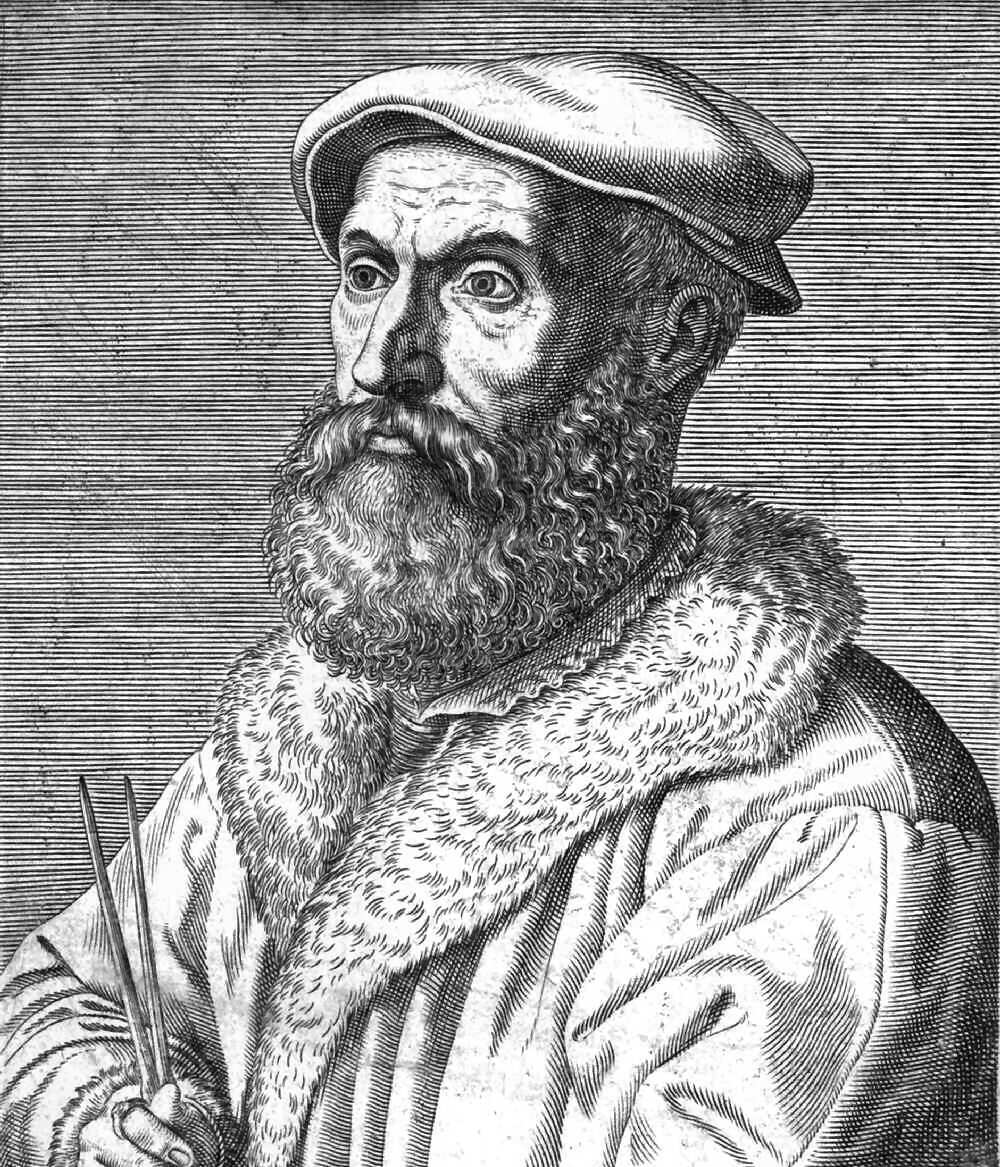
\includegraphics[width=0.555\linewidth]{pictures/Tartaglia}
			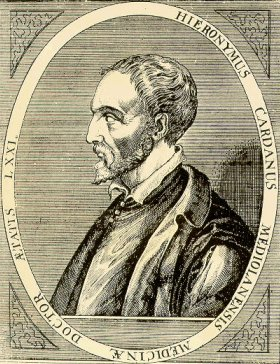
\includegraphics[width=0.5\linewidth]{pictures/Cardan}
			\caption{\small Tartaglia (esquerda) e Cardano, dois matemáticos do século 16 que descobriram soluções algébricas para equações do 3º grau envolvendo $\sqrt[2]{-1}$}
		\end{figure}
	\end{column}
	\begin{column}{.7\textwidth}
		\small
		\begin{itemize}
		\item No século 16, o matemático Tartaglia obteve, via manipulação algébrica, a seguinte expressão para as raízes da equação $x^3 = x$:
			\begin{equation}
				\frac{1}{\sqrt[2]{3}}\left( \sqrt[3]{\sqrt[2]{-1}} + \frac{1}{\sqrt[3]{\sqrt[2]{-1}}} \right)
			\end{equation}
		\item A princípio a equação não faz sentido, mas se manipulada com cuidado obtemos as raízes $0$, $1$ e $-1$ (todas reais).
		\item Os matemáticos da época perceberam que no caminho da obtenção de soluções reais, às vezes somos obrigados a passar por quantidades ``imaginárias''
		\item Isso elevou $\sqrt[2]{-1}$ ao status de \emph{número}, pois de repente se tornara útil
		\end{itemize}
	\end{column}
	\end{columns}

\end{frame}

\begin{frame}
	\frametitle{Números Complexos: $\mathbb{C}$}

	\begin{itemize}
		\item Agora precisamos dar um jeito de combinar os números reais com os números imaginários
		\item Como?
	\end{itemize}

\end{frame}

\begin{frame}
	\frametitle{Números Complexos: $\mathbb{C}$}

	\begin{itemize}
		\item Agora precisamos dar um jeito de combinar os números reais com os números imaginários
		\item Como?
		\item Podemos \emph{somar} números reais e números imaginários:
			\begin{equation}
			\begin{aligned}
				3 + 2\sqrt[2]{-1} \\
				42 - 8\sqrt[2]{-1} \\
				-20 + 30\sqrt[2]{-1} \\
				\dots
			\end{aligned}
			\end{equation}
	\end{itemize}

\end{frame}

\begin{frame}
	\frametitle{Números Complexos: $\mathbb{C}$}

	\begin{itemize}
		\item Pela última vez: vamos definir o conjunto dos números complexos
	\end{itemize}

\end{frame}

\begin{frame}
	\frametitle{Números Complexos: $\mathbb{C}$}

	\begin{itemize}
		\item Pela última vez: vamos definir o conjunto dos números complexos
		\item
			\begin{equation}
			\begin{aligned}
				\substack{\forall n ~\in~ \mathbb{R} \\ \forall m ~\in~ \mathbb{I}}: n + m \in \mathbb{C}
			\end{aligned}
			\end{equation}
	\end{itemize}

\end{frame}

\begin{frame}
	\frametitle{Números Complexos: $\mathbb{C}$}

	\begin{columns}[t]
	\begin{column}{.6\textwidth}
		\begin{figure}
			\def\Rcircle{		(-1cm,0) circle (0.5cm)}
			\def\Icircle{		(1cm,0) circle (0.5cm)}
			\def\Ccircle{		(0,0) circle (1.75cm)}

			% Now we can draw the sets:
			\begin{tikzpicture}
				\draw \Rcircle node			[shift={(0,0)}] 			{$\mathbb{R}$};
				\draw \Icircle node			[shift={(0,0)}]				{$\mathbb{I}$};
				\draw \Ccircle node			[shift={(0,1cm)}]	{$\mathbb{C}$};
			\end{tikzpicture}
			\caption{\small Diagrama de Venn dos conjuntos $\mathbb{R}, \mathbb{I}, \mathbb{C}$}
		\end{figure}
	\end{column}
	\begin{column}{.6\textwidth}
		\begin{itemize}
		\small
		\item Os números reais são a união dos números racionais com os números irracionais
		\item Pergunta: o mesmo vale para os complexos? Os números complexos são a união dos números reais com os números imaginários?
		\end{itemize}
	\end{column}
	\end{columns}

\end{frame}

\begin{frame}
	\frametitle{Números Complexos: $\mathbb{C}$}

	\begin{columns}[t]
	\begin{column}{.6\textwidth}
		\begin{figure}
			\def\Rcircle{		(-1cm,0) circle (0.5cm)}
			\def\Icircle{		(1cm,0) circle (0.5cm)}
			\def\Ccircle{		(0,0) circle (1.75cm)}

			% Now we can draw the sets:
			\begin{tikzpicture}
				\draw \Rcircle node			[shift={(0,0)}] 			{$\mathbb{R}$};
				\draw \Icircle node			[shift={(0,0)}]				{$\mathbb{I}$};
				\draw \Ccircle node			[shift={(0,1cm)}]	{$\mathbb{C}$};
			\end{tikzpicture}
			\caption{\small Diagrama de Venn dos conjuntos $\mathbb{R}, \mathbb{I}, \mathbb{C}$}
		\end{figure}
	\end{column}
	\begin{column}{.6\textwidth}
		\begin{itemize}
		\small
		\item Os números reais são a união dos números racionais com os números irracionais
		\item Pergunta: o mesmo vale para os complexos? Os números complexos são a união dos números reais com os números imaginários?
		\item {\color{red}Não! Por exemplo, $2 + 3i$ não é real nem imaginário!}
		\end{itemize}
	\end{column}
	\end{columns}

\end{frame}

\begin{frame}
	\frametitle{Números Complexos: $\mathbb{C}$}

	\begin{itemize}
		\item OK! Mas o que nos impede de inventar outros números? Quando essa brincadeira dos conjuntos numéricos acaba?
	\end{itemize}

\end{frame}

\begin{frame}
	\frametitle{Números Complexos: $\mathbb{C}$}

	\begin{columns}[t]
	\begin{column}{.3\textwidth}
		\begin{figure}
			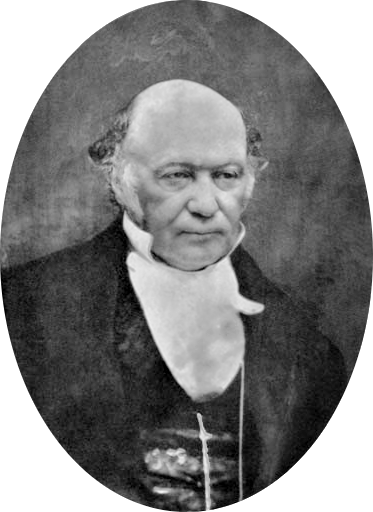
\includegraphics[width=0.9\linewidth]{pictures/Hamilton}
			\caption{\small Hamilton extendeu os números complexos acrescentando mais duas raízes (distintas) de $-1$: $i^2 = j^2 = k^2 = ijk = -1$}
		\end{figure}
	\end{column}
	\begin{column}{.7\textwidth}
		\small
		\begin{itemize}
		\item OK! Mas o que nos impede de inventar outros números? Quando essa brincadeira dos conjuntos numéricos acaba?
		\item Nada nos impede!
		\item Mas tem um detalhe: agora não é mais \emph{necessário} definir novos conjuntos
		\item Por quê?
		\end{itemize}
	\end{column}
	\end{columns}

\end{frame}

\begin{frame}
	\frametitle{Números Complexos: $\mathbb{C}$}

	\begin{columns}[t]
	\begin{column}{.3\textwidth}
		\begin{figure}
			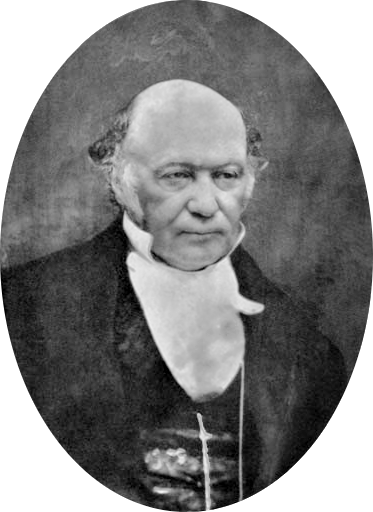
\includegraphics[width=0.9\linewidth]{pictures/Hamilton}
			\caption{\small Hamilton extendeu os números complexos acrescentando mais duas raízes (distintas) de $-1$: $i^2 = j^2 = k^2 = ijk = -1$}
		\end{figure}
	\end{column}
	\begin{column}{.7\textwidth}
		\small
		\begin{itemize}
		\item OK! Mas o que nos impede de inventar outros números? Quando essa brincadeira dos conjuntos numéricos acaba?
		\item Nada nos impede!
		\item Mas tem um detalhe: agora não é mais \emph{necessário} definir novos conjuntos
		\item Por quê?
		\item {\color{red}Os números complexos são \emph{algebricamente fechados}}
		\item Toda equação polinomial tem solução nos números complexos!
		\end{itemize}
	\end{column}
	\end{columns}

\end{frame}

\begin{frame}
	\frametitle{Resumo do que vimos até agora: $\mathbb{N}, \mathbb{Z}, \mathbb{Q}, \mathbb{R}, \mathbb{I}, \mathbb{C}$}

	\begin{itemize}
		\item Obtemos os números inteiros ($\mathbb{Z}$) generalizando a subtração para aceitar números negativos
		\item Obtemos os números racionais ($\mathbb{Q}$) generalizando a divisão para aceitar números fracionários
		\item Obtemos os números reais ($\mathbb{R}$) preenchendo as lacunas dos números racionais
		\item Obtemos os números imaginários ($\mathbb{I}$) generalizando a raiz quadrada ($\sqrt[2]{2}$) para aceitar raizes de números negativos
		\item Obtemos os números complexos ($\mathbb{C}$) generalizando a adição para aceitar somas entre números reais e números imaginários
	\end{itemize}

\end{frame}

\end{document}